\documentclass{article}
\setlength{\oddsidemargin}{0.25 in}
\setlength{\evensidemargin}{-0.25 in}
\setlength{\topmargin}{-0.6 in}
\setlength{\textwidth}{6.5 in}
\setlength{\textheight}{8.5 in}
\setlength{\headsep}{0.75 in}
\setlength{\parindent}{0 in}
\setlength{\parskip}{0.1 in}

% ===== PACKAGES =====
\usepackage{xcolor, graphicx, wrapfig}
\usepackage{url, hyperref, dirtree, listings}
\usepackage{courier, lipsum}
\usepackage{amsmath,amssymb}
\usepackage{color}
\usepackage{subfigure}
\usepackage{mdframed}
\usepackage{changepage}
\newmdenv[
  topline=false,
  bottomline=false,
  skipabove=\topsep,
  skipbelow=\topsep
]{siderules}
\renewcommand{\abstractname}{}

% ===== NEW COMMAND =====
\definecolor{light-gray}{gray}{0.95}
\newcommand{\code}[1]{\colorbox{light-gray}{\texttt{#1}}}
\lstset{basicstyle=\footnotesize\ttfamily,breaklines=true}

% ===== VARIABLES =====
\def \R{\mathbb{R}}
\def \Pr{\mathbb{P}}
\def \D{{\rm D}}
\def \N{{\rm N}}
\def \xx{{\boldsymbol{\rm x}}}
\def \y{{\rm y}}




% ===== HEADER BOX =====
\newcommand{\lecture}[2]{
\pagestyle{myheadings}
\thispagestyle{plain}
\newpage
\noindent
\begin{center}
\rule{\textwidth}{1.6pt}\vspace*{-\baselineskip}\vspace*{2pt} % Thick horizontal line
\rule{\textwidth}{0.4pt}\\[1\baselineskip] % Thin horizontal line
\vbox{\vspace{2mm}
\hbox to 6.28in { {\bf CS 760: Machine Learning} \hfill Fall 2020 }
\vspace{4mm}
\hbox to 6.28in { {\Large \hfill #1  \hfill} }
\vspace{4mm}
\hbox to 6.28in { {\scshape Authors:}  #2 \hfill }}
\vspace{-2mm}
\rule{\textwidth}{0.4pt}\vspace*{-\baselineskip}\vspace{3.2pt} % Thin horizontal line
\rule{\textwidth}{1.6pt}\\[\baselineskip] % Thick horizontal line
\end{center}
\vspace*{4mm}
}



% =============== DOCUMENT ===============
\begin{document}
\lecture{Face Mask Detection}{Zijie Zhang}

\begin{center}
{\Large {\sf GO GREEN. AVOID PRINTING, OR PRINT 2-SIDED OR MULTIPAGE.}}
\end{center}

\begin{abstract}
Write your abstract here
\end{abstract}

\section{Introduction}
With the global outbreak of COVID-19, it's even more important to have some policy to mitigate risk. For public safety and health, people are recommended to wear face masks and coverings to control the spread of the COVID-19.

In hospitals and various COVID-19 testing places. If only people wearing masks are allowed to enter, the risk of infection for doctors and staff can be reduced. However, if a potential COVID-19 infected person who is not wearing a mask suddenly appears, there is a high risk of infection in face-to-face communication.

At many intersections, pedestrians will gather briefly while waiting for traffic lights. At this time, the risk of COVID-19 spreading among the population is high. But it is impossible to hire a person to stay at the intersection and remind pedestrians to wear masks.

Similarly, requiring Uber drivers and passengers to wear masks at all times can also effectively reduce the spread of the COVID-19. However, it is impossible to supervise the wearing of masks on moving vehicles in real time.

There are many application scenarios such as this. If it is all supervised by manpower, the investment cost is high, and the health risks of the staff are also high.

Therefore, the need for artificial intelligence to determine the wearing of masks came into being. The main idea of this project is to construct a classifier to judge whether the photo cropped from the face detector is wearing a mask.

\section{Related/Similar work}
This project is mainly inspired by \textbf{Baidu AI development platform - mask wearing detection products}.

\url{https://ai.baidu.com/tech/body/driver}


Related/Similar work:
\begin{enumerate}
  \item \url{https://github.com/AIZOOTech/FaceMaskDetection}
  \item \url{https://github.com/chandrikadeb7/Face-Mask-Detection}
  \item \url{https://arxiv.org/abs/2003.09093}
\end{enumerate}

\section{Dataset}

  \subsection{Source}
  The data comes from the following sources:
  \begin{enumerate}
    \item \textbf{Real-World Masked Face Dataset, RMFD}\\
          \url{https://github.com/X-zhangyang/Real-World-Masked-Face-Dataset}
    \item \textbf{CASIA-WebFace-Dataset}
  \end{enumerate}
  \subsection{Description}
  \begin{enumerate}
    \item The dataset contains 3400 images, which belong to two categories:
          \begin{enumerate}
            \item \textbf{with\_mask: 1470}
            \item \textbf{without\_mask: 1930}
          \end{enumerate}

    \item Classes:\{'with\_mask', 'without\_mask'\}
    
    \item The directory structure:
          \DTsetlength{0.2em}{1em}{0.2em}{1pt}{3pt}
          \dirtree{%
          .1 .
          .2 dataset.
          .3 with\_mask \ldots{} \begin{minipage}[t]{5cm}
            1470 images{.}
            \end{minipage}.
          .3 without\_mask \ldots{} \begin{minipage}[t]{5cm}
            1930 images{.}
            \end{minipage}.
          }
  \end{enumerate}


\section{Approach}

  \subsection{Pre-processing}
  \begin{enumerate}
    \item Since the shapes of the images in the data set are not the same, the first step of preprocessing is to resize all images to the same shape.(180x180)
    \item Data augmentation:\\
          Due to the small sample size of the data set, over-fitting is prone to occur. Therefore, the operation of data augmentation was added. Generate some effective new data on the basis of existing data by using random transformation. This helps expose the model to more aspects of the data.

          \begin{enumerate}
            \item ColorJitter
            \item RandomRotation
            \item RandomVerticalFlip
            \item RandomHorizontalFlip
          \end{enumerate}
    \item For each RGB image, it has three channels. We can convert it to a [3, 180, 180] \textbf{Tensor}.
    \item For each element in the tensor, its range is [0,255]. We should normalize them.
    \item Data preview:
  \end{enumerate}
  \begin{center}
    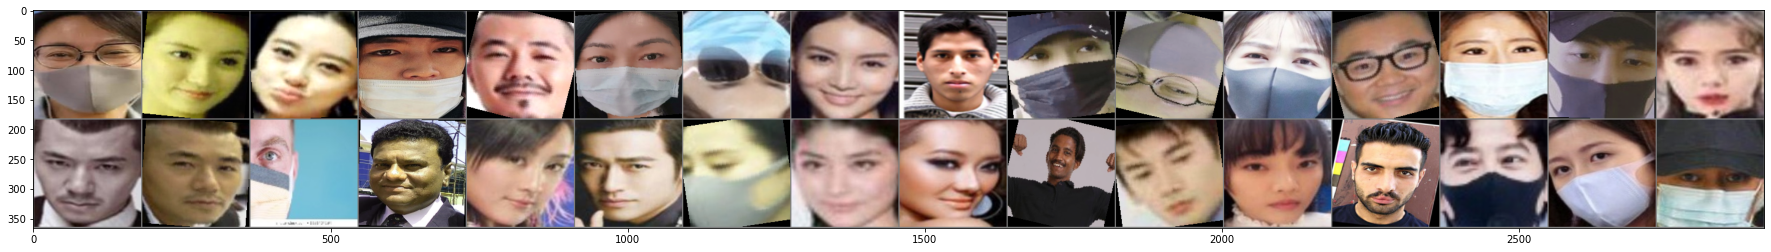
\includegraphics[width=15cm]{preview.png}
  \end{center}
  \begin{lstlisting}
  Transforms = transforms.Compose([
      transforms.Resize((IMAGE_HEIGHT, IMAGE_WIDTH)),
      transforms.RandomApply(torch.nn.ModuleList([
          transforms.ColorJitter(brightness=0.1, contrast=0.1, saturation=0.1, hue=0.1),
          transforms.RandomRotation(degrees=15),
      ]), p=0.3),
      transforms.RandomVerticalFlip(p=0.1),
      transforms.RandomHorizontalFlip(p=0.1),
      transforms.ToTensor(),
      transforms.Normalize((0.5, 0.5, 0.5), (0.5, 0.5, 0.5))
  ])
  \end{lstlisting}
  
  \subsection{Neural Networks Method}
  Generally, Convolutional Neural Networks (CNN) are complex feed forward neural networks. CNNs are used for image classification and recognition because of its high accuracy.

  So the first method is Neural Networks.
  \begin{figure}[!htbp]
    \minipage{0.24\textwidth}
      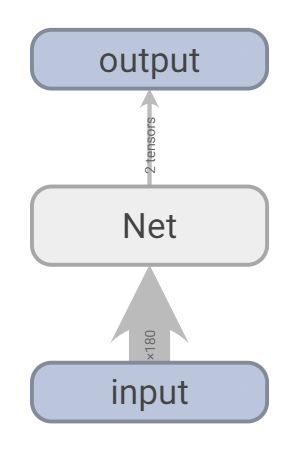
\includegraphics[width=4cm]{structure1.JPG}
    \endminipage\hfill
    \minipage{0.24\textwidth}
      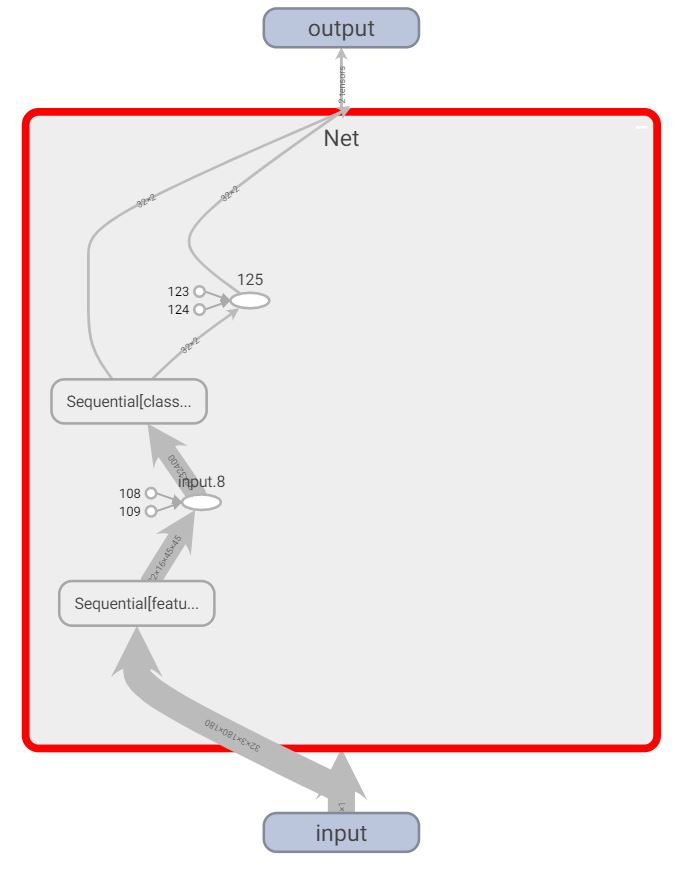
\includegraphics[width=4cm]{structure2.JPG}
    \endminipage\hfill
    \minipage{0.24\textwidth}
      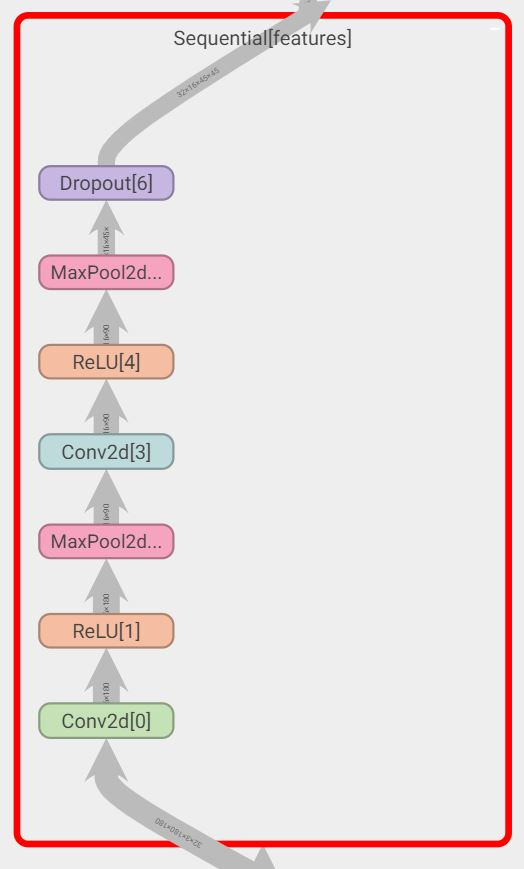
\includegraphics[width=4cm]{structure4.JPG}
    \endminipage\hfill
    \minipage{0.24\textwidth}
      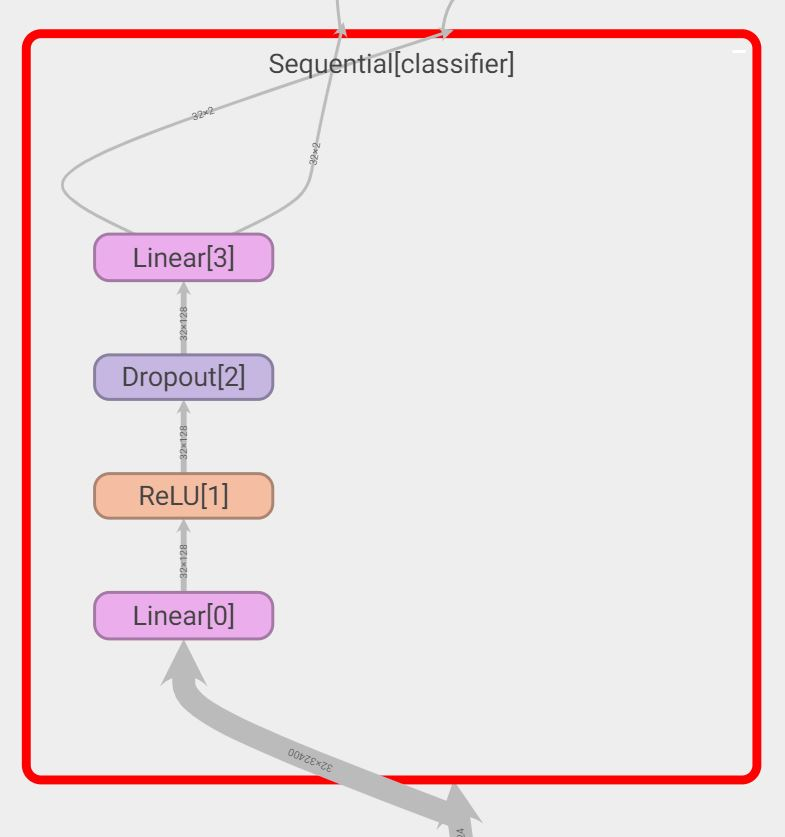
\includegraphics[width=4cm]{structure3.JPG}
    \endminipage
    \end{figure}
  \begin{enumerate}
    \item The main structure of the neural network consists of two parts: Feature learning and classifier.
    \item The first part includes two \textbf{Conv2d} layer.
    \item The second part is a Full-Connected Network.
  \end{enumerate}
  \begin{lstlisting}
  Net(
    (features): Sequential(
      (0): Conv2d(3, 16, kernel_size=(3, 3), stride=(1, 1), padding=(1, 1))
      (1): ReLU(inplace=True)
      (2): MaxPool2d(kernel_size=(2, 2), stride=(2, 2), padding=0, dilation=(1, 1), ceil_mode=False)
      (3): Conv2d(16, 16, kernel_size=(3, 3), stride=(1, 1), padding=(1, 1))
      (4): ReLU(inplace=True)
      (5): MaxPool2d(kernel_size=(2, 2), stride=(2, 2), padding=0, dilation=(1, 1), ceil_mode=False)
      (6): Dropout(p=0.2, inplace=False)
    )
    (classifier): Sequential(
      (0): Linear(in_features=32400, out_features=128, bias=True)
      (1): ReLU(inplace=True)
      (2): Dropout(p=0.2, inplace=False)
      (3): Linear(in_features=128, out_features=2, bias=True)
    )
  )
  \end{lstlisting}

  \subsection{Nearest Neighbors Algorithm}
  Considering the use of K-NN algorithm to achieve face recognition, we can try to use K-NN for mask wearing recognition.

  Based on the previous preprocessing, flatten each Tensor into a 1-dimension vector.

  Choose algorithm = 'kd\_tree' to speed up. Implement with parameters:\begin{lstlisting}
    n_neighbors = 15, weight = 'distance', metric='euclidean'
  \end{lstlisting}
  For a new image after preprocessing, we will gave a point in the 32400-dimension vector space. Calculate the Euclidean distance from this point to every known point. The predicted value of this unknown point is obtained by weighted voting of the 15 known points closest to it.

  \subsection{Random Forest Algorithm}
  As we all know, decision trees can be very sensitive to the specific data we observe. In fact, they can be quite biased, and tend to overfit.

  After randomly slicing the original data set, generate a decision tree on each data set after the split. Use information entropy as the criterion for selecting nodes.

  After generating a hundred decision trees like this, for a new image after preprocessing, every decision tree will give a prediction. Choose the class with the most votes as the predicted value of the new image.

  \subsection{Packages}
    (1) pytorch
    (2) sklearn
    (3) PIL
    (4) numpy
    (5) opencv

\section{Results}

  \subsection{Description of experiments}
  For the above three methods, after randomly slicing the original data set at a ratio of 0.2, train on the training set to obtain accuracy on the test set.
  \begin{enumerate}
    \item \textbf{Neural Networks}:
          \begin{enumerate}
            \item Accuracy of the network on the test images: 92 \%.
            \item Accuracy of with\_mask : 95 \%.
            \item Accuracy of without\_mask : 91 \%.
          \end{enumerate}
    \item \textbf{Nearest Neighbors}:\begin{lstlisting}
[ Nearest Neighbors ]
      classification report on the test set
      done in 22.212s
                    precision    recall  f1-score   support

                0       0.92      0.73      0.81       294
                1       0.82      0.95      0.88       386

         accuracy                           0.86       680
        macro avg       0.87      0.84      0.85       680
     weighted avg       0.87      0.86      0.85       680
    \end{lstlisting}
    \item \textbf{Random Forest}:\begin{lstlisting}
[ Random Forest ]
      classification report on the test set
      done in 0.061s
                    precision    recall  f1-score   support

                0       0.92      0.84      0.88       294
                1       0.88      0.95      0.91       386

         accuracy                           0.90       680
        macro avg       0.90      0.89      0.90       680
     weighted avg       0.90      0.90      0.90       680
    \end{lstlisting}

  \end{enumerate}
  \subsection{Comparisons}
  \textbf{Training time:}

  The neural network model executed 15 epochs, with a long training time and many parameters. In comparison, the nearest neighbor algorithm has almost no training time. The training time of random forest algorithm is moderate.

  \textbf{Performance:}

  Although the kd\_tree algorithm is used, the performance of the nearest neighbor algorithm is still very bad, which is determined by its principle. The larger the data set, the greater the computational overhead.

  The performance of neural networks and random forests is very good. The scale of the neural network is determined before training, and the depth of each decision tree in the random forest is not very large, so the results can be quickly obtained.

  \textbf{Generalization:}
  The neural network model has many parameters and is very complex. For the problem of mask recognition, if there is no overfitting, its generalization ability is very strong.

  However, for traditional machine learning algorithms, the model complexity of k-nearest neighbors is not high, and it is difficult to effectively learn the laws behind the data.

  For the random forest algorithm, it is an embedded algorithm. The data space of each decision tree is different, so that the underlying laws of the data can be learned from multiple angles.
  
  In the ideal situation where the classification strength of a single decision tree is as high as possible and the correlation between decision trees is as small as possible, the random forest algorithm has strong generalization ability.
  \subsection{Results}
  In general, for the image classification problem, the neural network model has great advantages in accuracy and generalization ability.

  The K-nearest neighbor algorithm is worth studying in terms of metric selection. Its performance is weak and may perform better in a small sample space.

  The performance of the random forest algorithm is close to neural network. The process of using information entropy to select features to generate a decision tree is very efficient.

\section{Conclusions and Future Work}


\section{References}


\end{document} 
































